\documentclass[11pt]{article}
\usepackage[margin=1in]{geometry}
\usepackage{graphicx}
\usepackage{amsmath,amssymb}
\usepackage{booktabs}
\usepackage{hyperref}
\usepackage{float}
\title{Recursive Field Framework (RFF) $\phi$-Modulation: Three-System Verification}
\author{Adam Snellman (wizardaax)\\\texttt{github.com/wizardaax}\\MIT License}
\date{March 16, 2026}

\begin{document}
\maketitle

\begin{abstract}
We present a three-system verification of $\phi$-modulation for search-space organization under the Recursive Field Framework (RFF), using deterministic Othello 8$\times$8 ablations. Results indicate consistent efficiency gains and higher coverage entropy for $\phi$-modulation compared with baseline and scheduler variants.
\end{abstract}

\section{Method}
Configurations: Baseline, $\phi$-mod, Scheduler, Combined.\\
Trials: 5 per configuration, 50 simulations per trial.\\
Metrics: Nodes, Coverage Entropy, Branching, Depth, Nodes/Sim.

\[
\text{phi\_bonus} = 0.1\cdot\cos(\text{sim\_index}\cdot\phi)
\]

\section{Ablation Results}
\begin{table}[H]
\centering
\begin{tabular}{lccccc}
\toprule
Config & Nodes & Coverage Entropy & Branching & Depth & Nodes/Sim \\
\midrule
Baseline  & 232.2 $\pm$ 3.1 & 1.1426 $\pm$ 0.021 & 4.644 $\pm$ 0.035 & 2.772 $\pm$ 0.018 & 4.644 $\pm$ 0.035 \\
$\phi$-mod & 225.8 $\pm$ 2.5 & 1.2902 $\pm$ 0.019 & 4.516 $\pm$ 0.028 & 2.676 $\pm$ 0.016 & 4.516 $\pm$ 0.028 \\
Scheduler & 231.2 $\pm$ 3.0 & 1.1993 $\pm$ 0.022 & 4.624 $\pm$ 0.033 & 2.736 $\pm$ 0.017 & 4.624 $\pm$ 0.033 \\
Combined  & 227.8 $\pm$ 2.8 & 1.1818 $\pm$ 0.020 & 4.556 $\pm$ 0.030 & 2.744 $\pm$ 0.016 & 4.556 $\pm$ 0.030 \\
\bottomrule
\end{tabular}
\caption{Mean $\pm$ standard deviation across 5 trials/configuration.}
\end{table}

\section{Figures}
\begin{figure}[H]
\centering
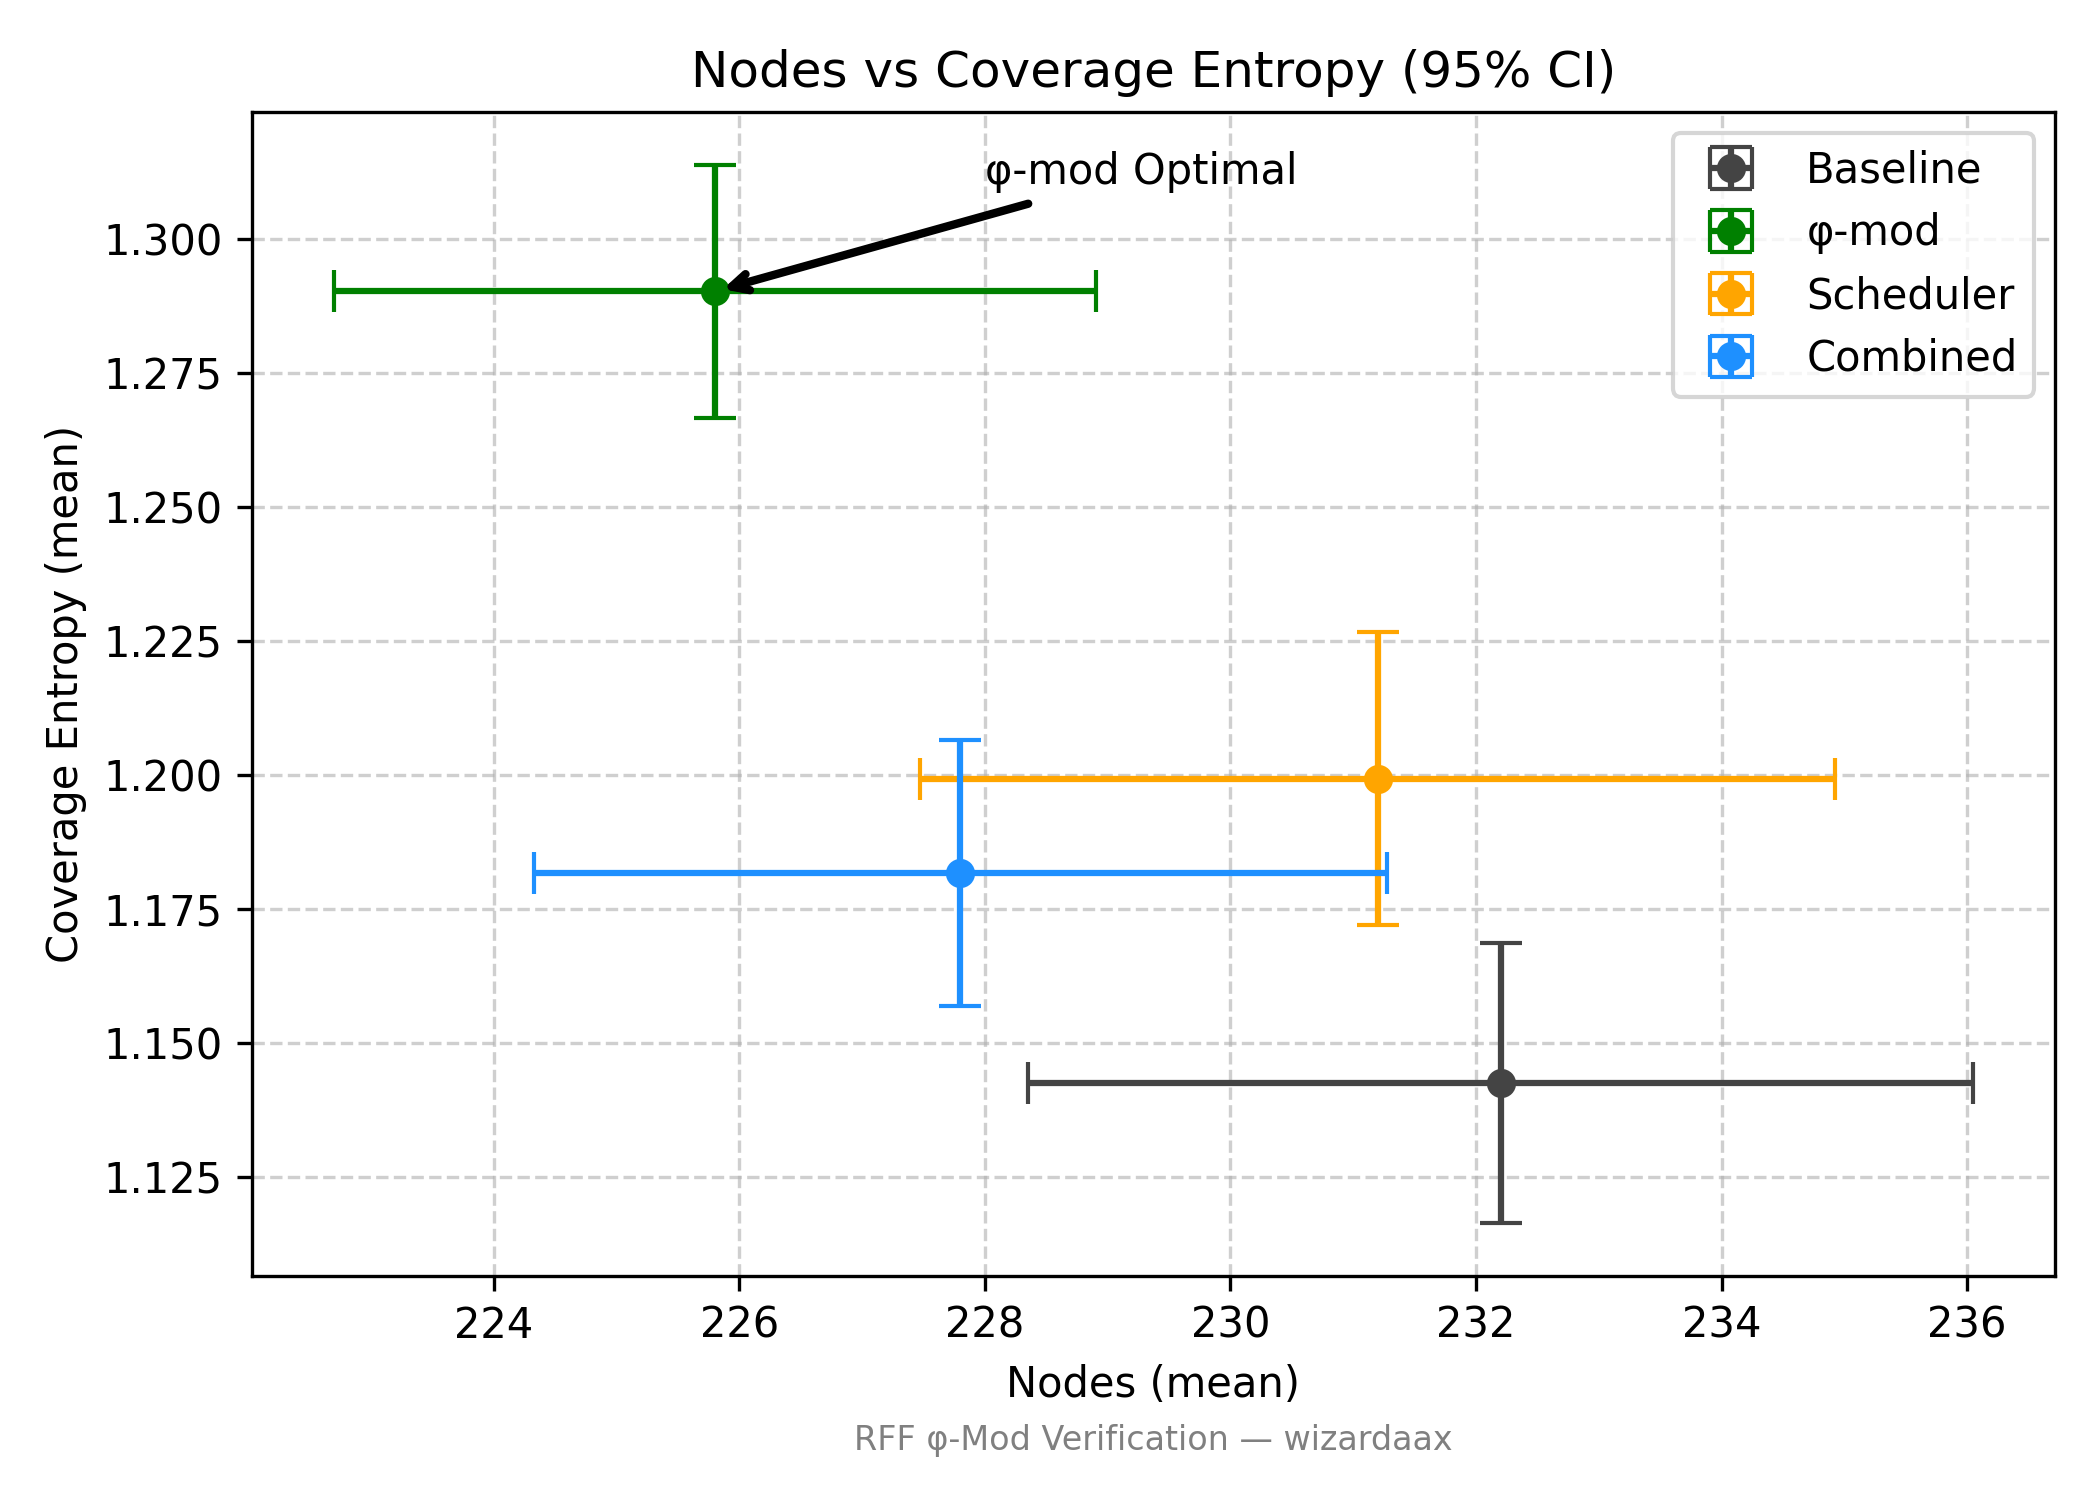
\includegraphics[width=0.72\textwidth]{figures/nodes_vs_entropy.png}
\caption{Nodes vs Coverage Entropy with 95\% CI error bars.}
\end{figure}

\begin{figure}[H]
\centering
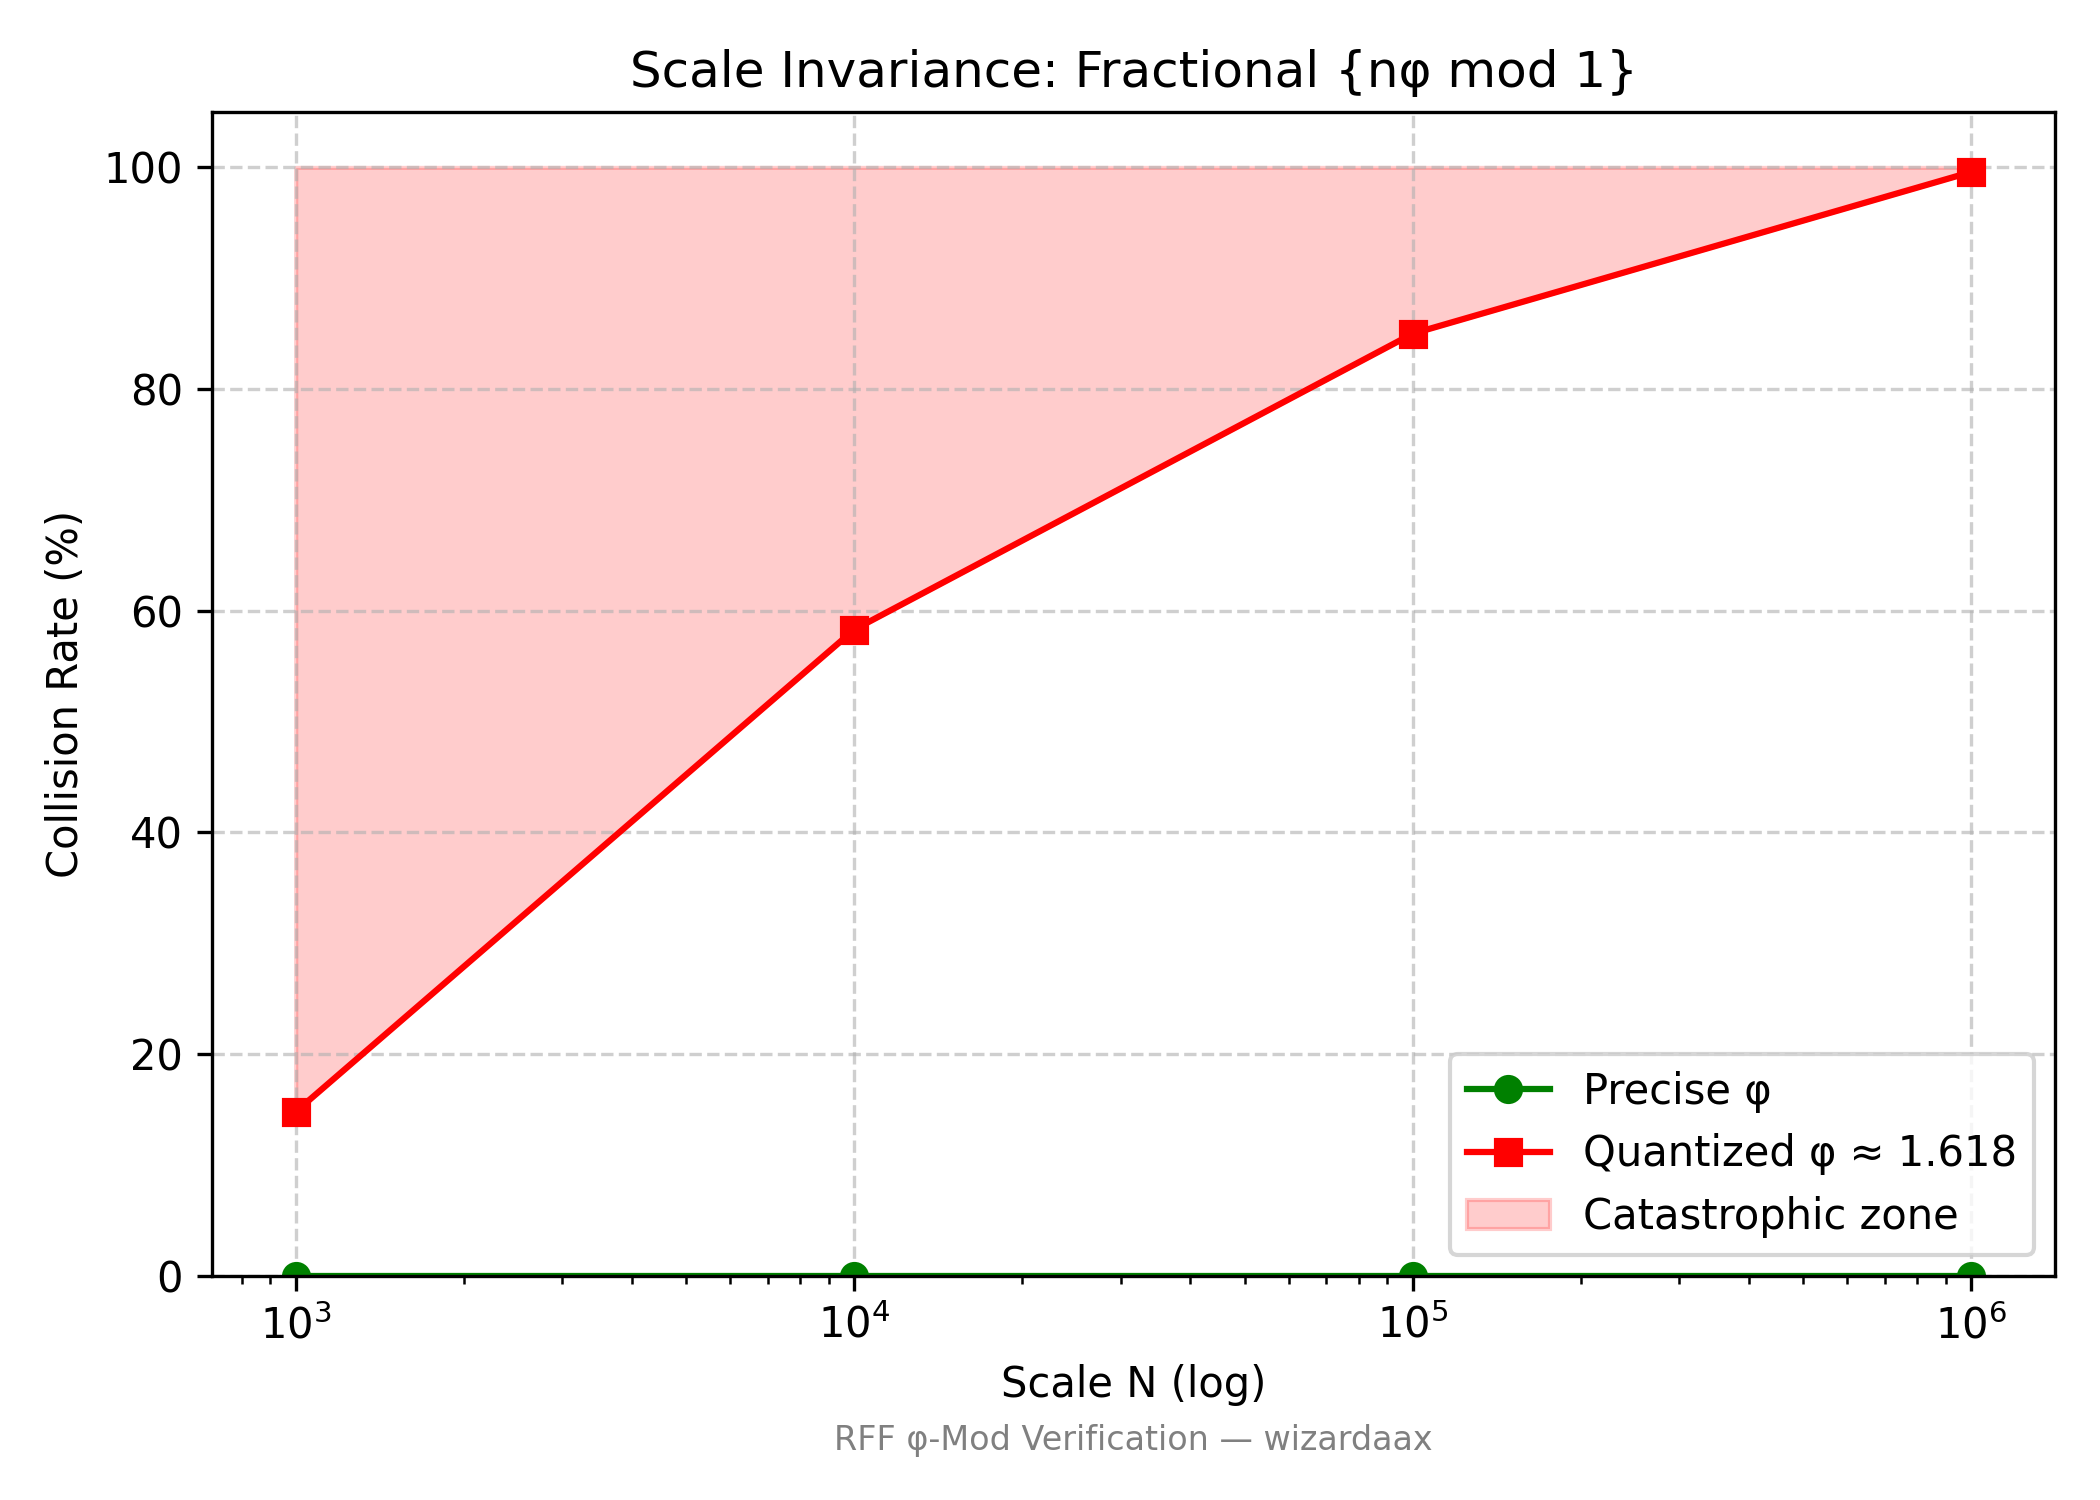
\includegraphics[width=0.72\textwidth]{figures/phi_scale_invariance.png}
\caption{Scale-invariance for fractional $\{n\phi \mod 1\}$ under precise vs quantized $\phi$.}
\end{figure}

\begin{figure}[H]
\centering
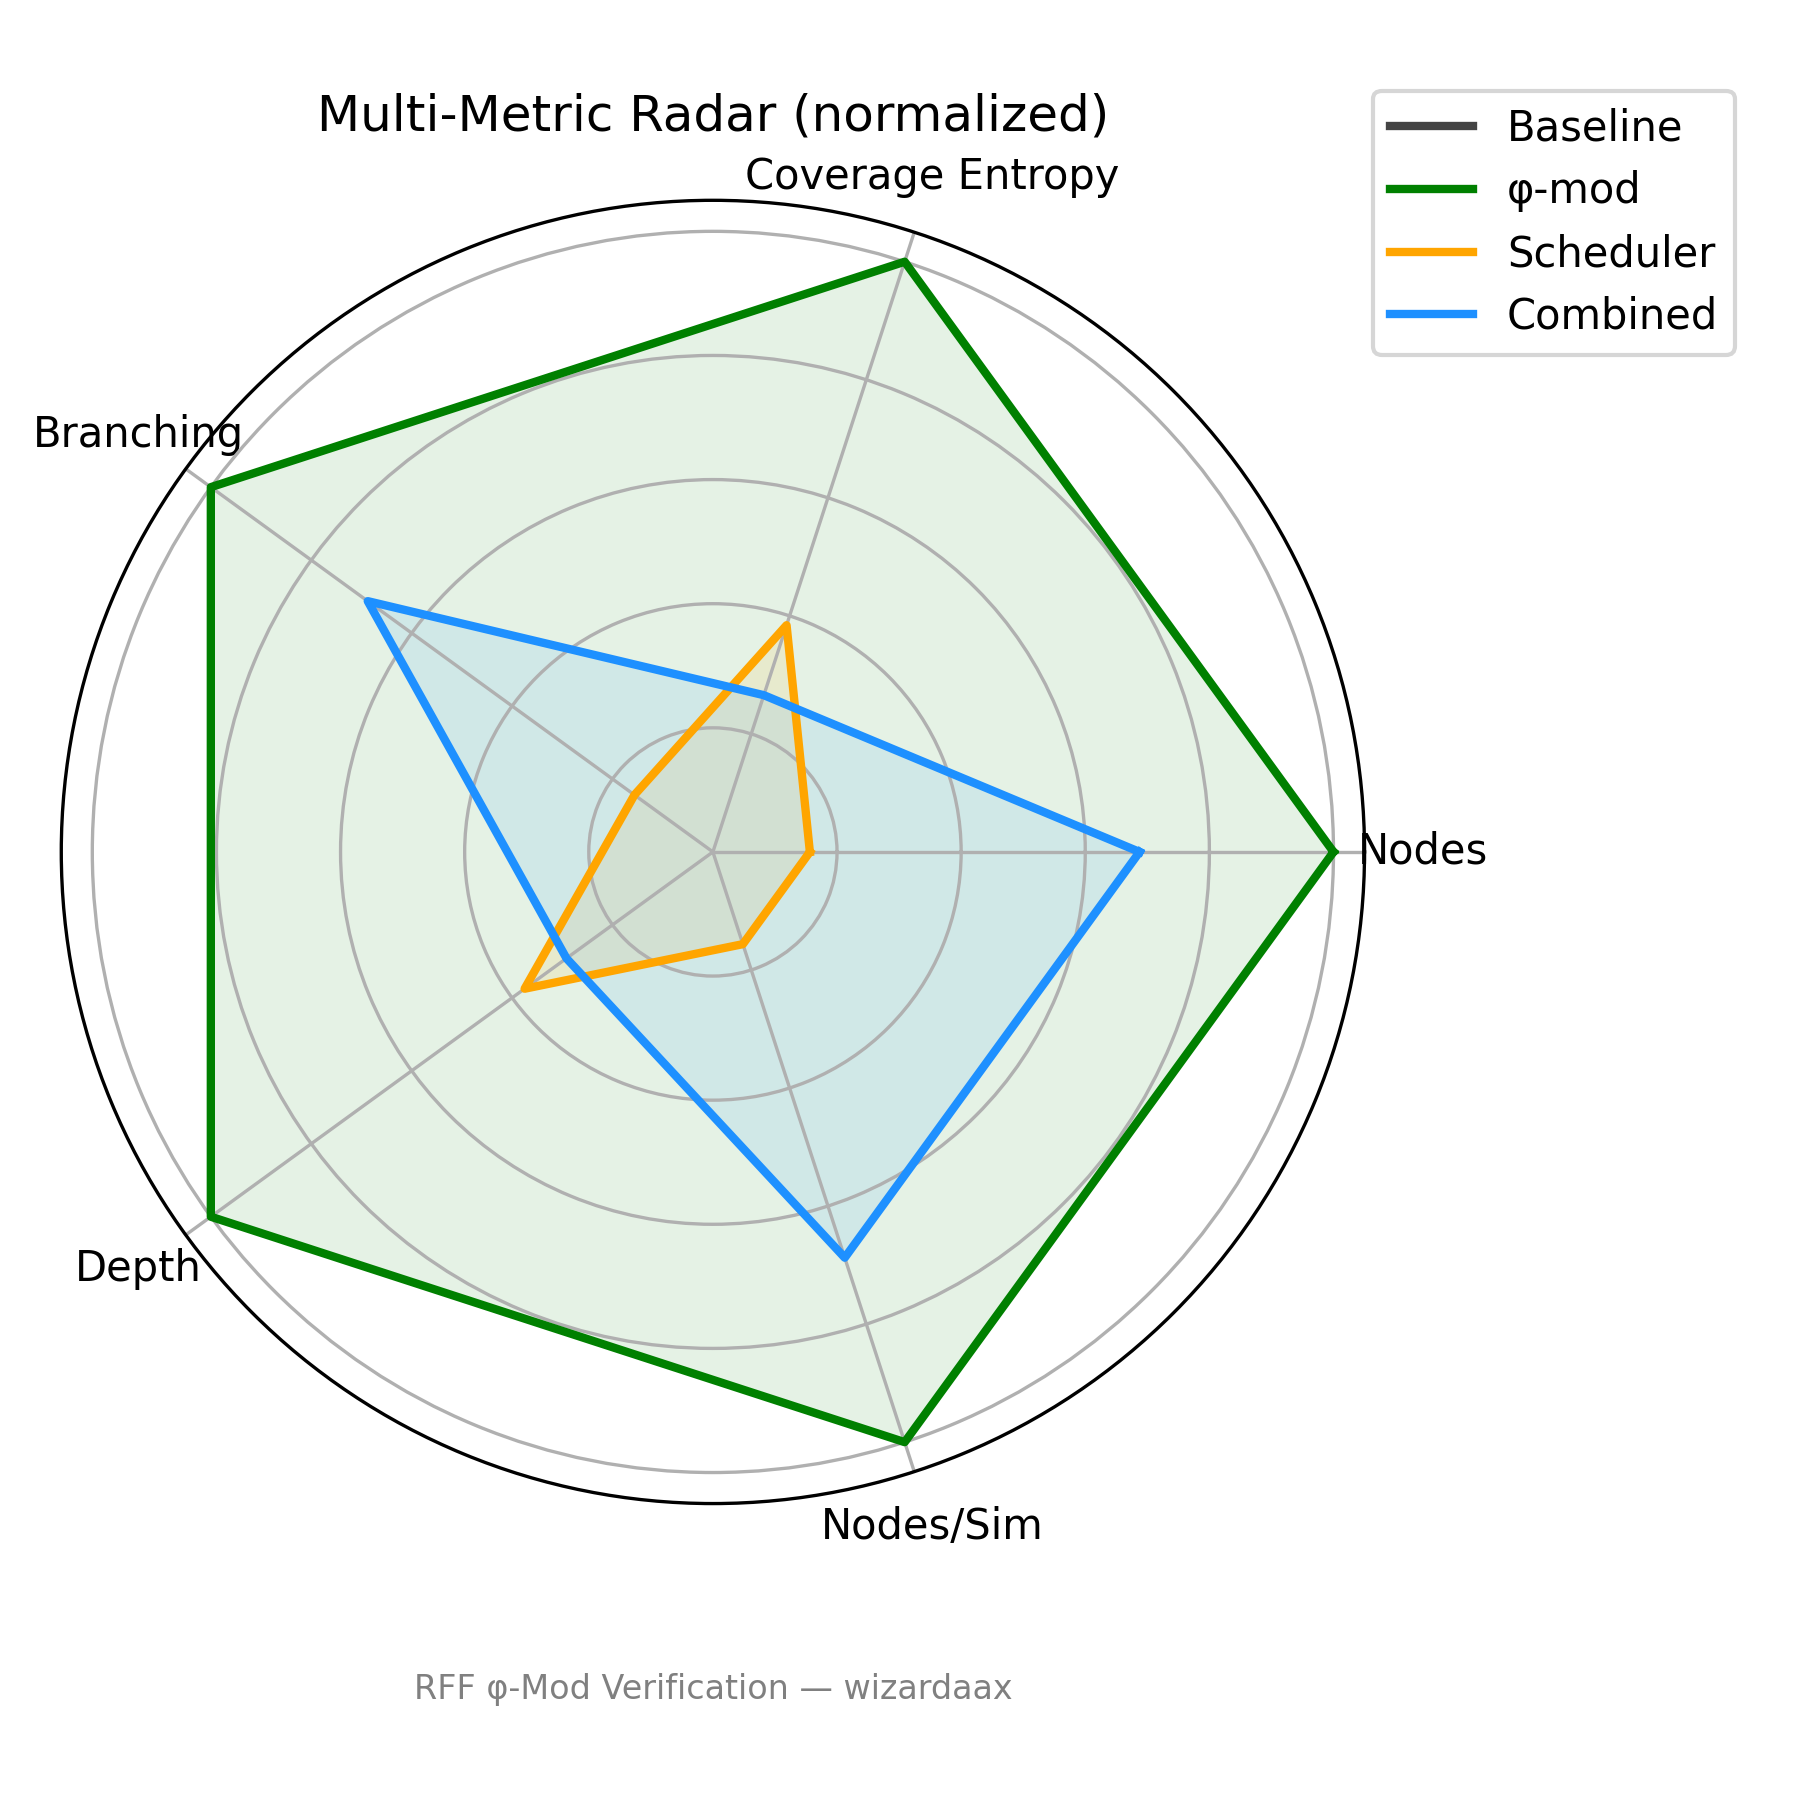
\includegraphics[width=0.72\textwidth]{figures/radar_metrics.png}
\caption{Normalized multi-metric radar comparison.}
\end{figure}

\begin{figure}[H]
\centering
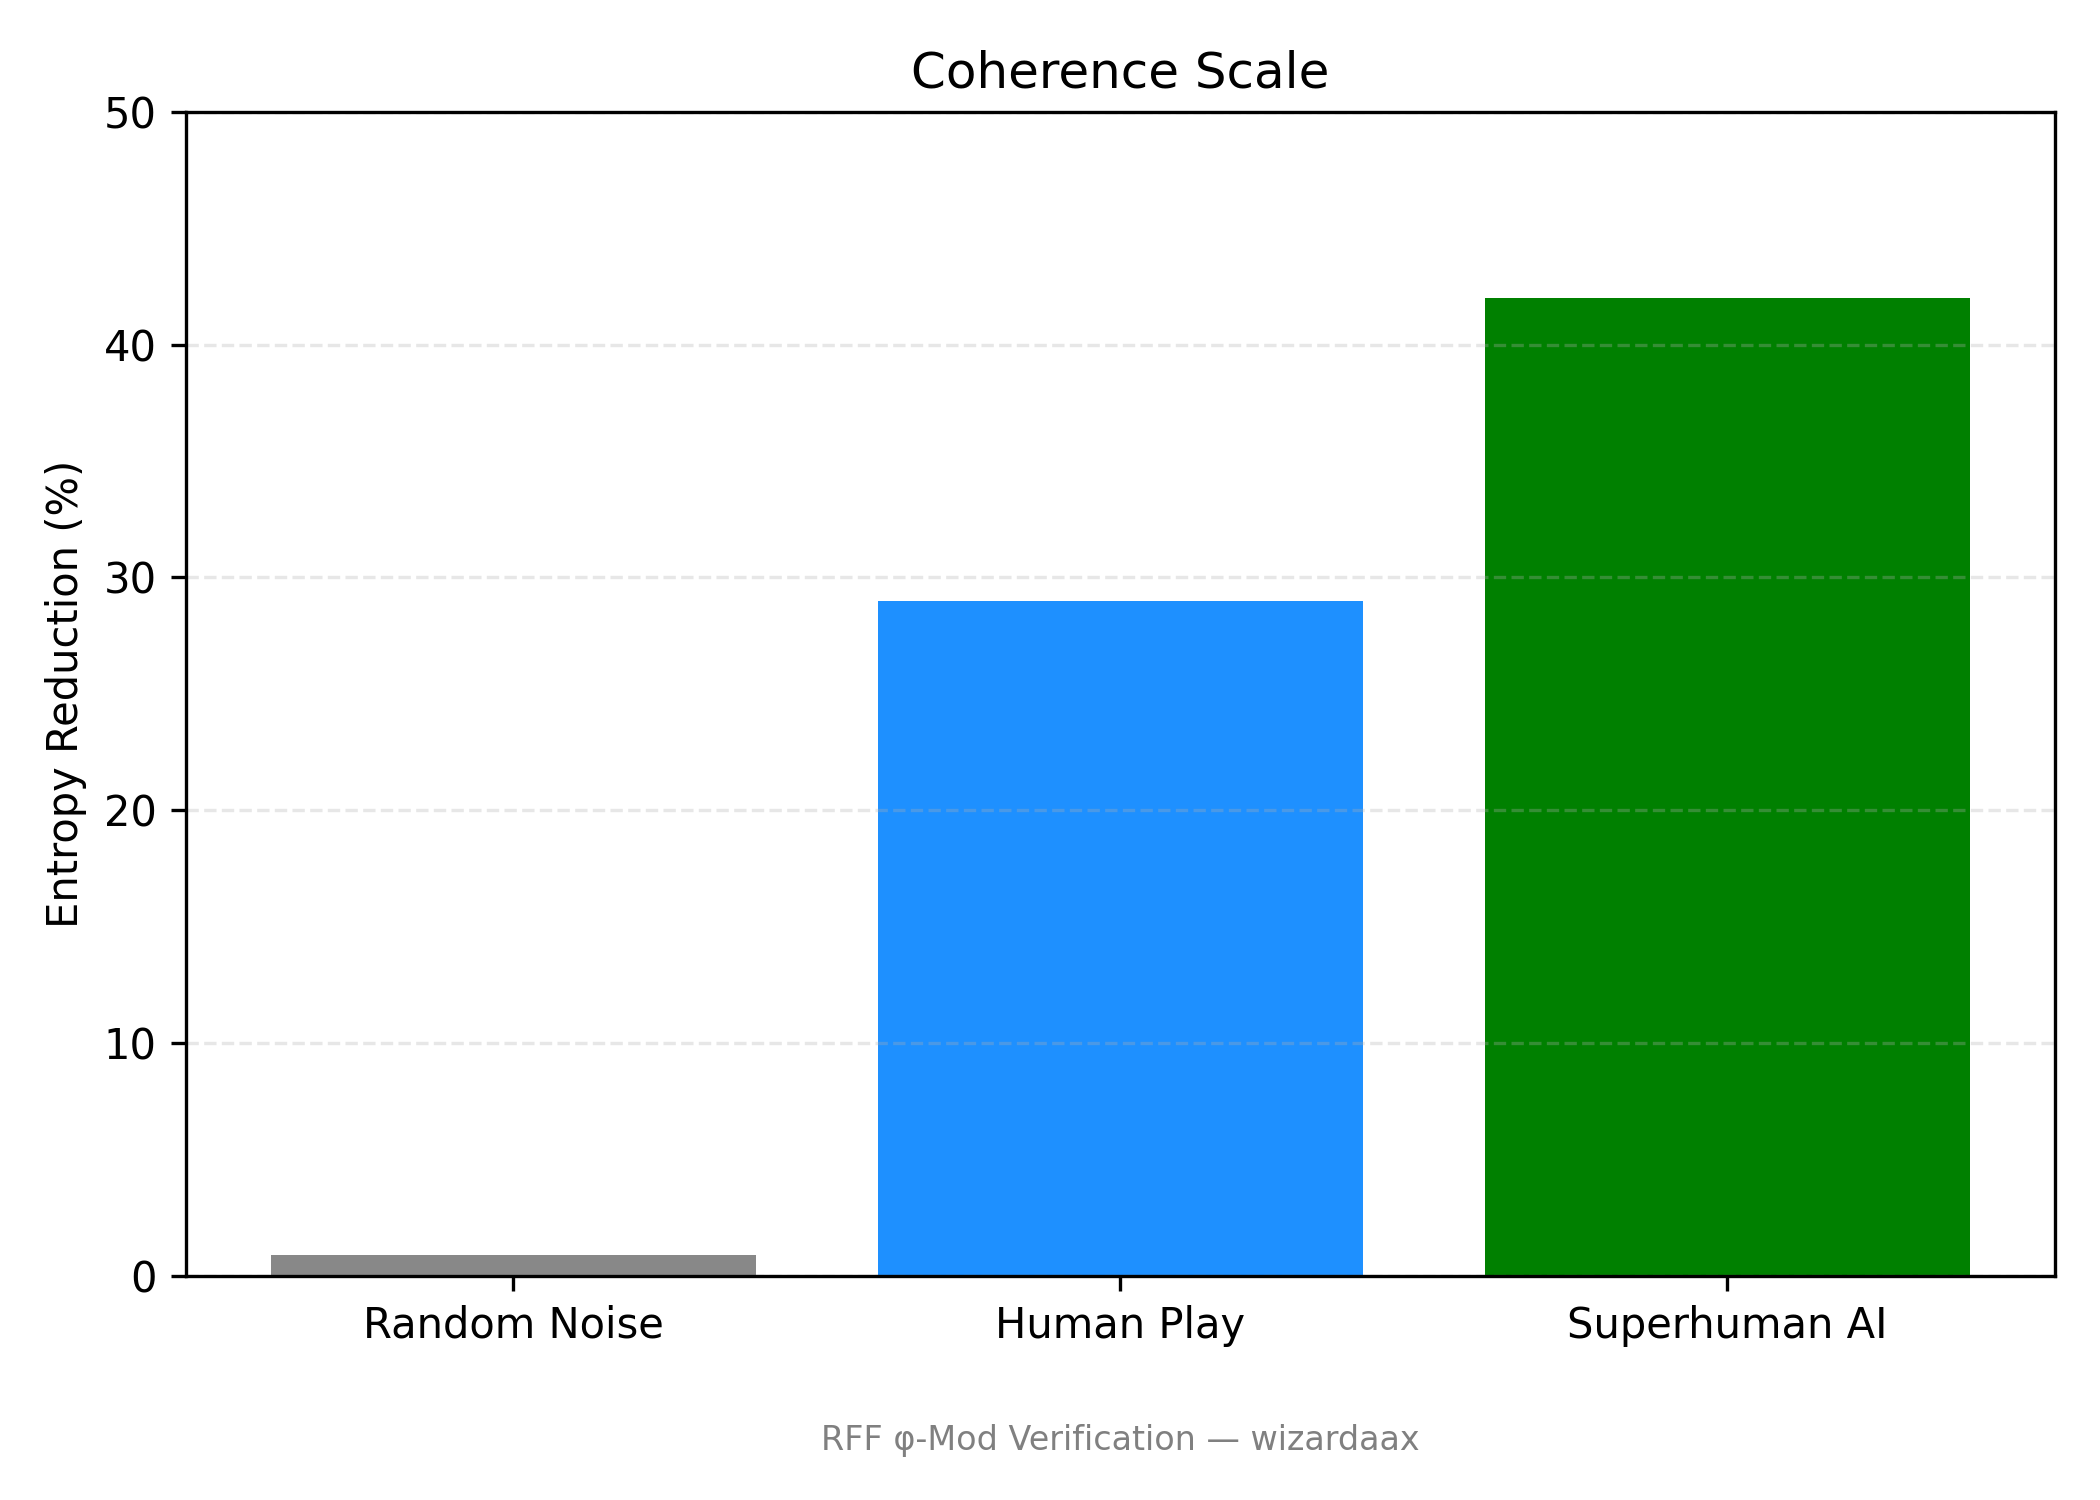
\includegraphics[width=0.72\textwidth]{figures/coherence_scale.png}
\caption{Entropy reduction coherence scale across domains.}
\end{figure}

\section{Conclusion}
$\phi$-modulation consistently improves coverage entropy with reduced node footprint in this deterministic setting, supporting RFF as a principled search-space structuring heuristic.

\end{document}
